\addbibresource{reference.bib}

\chapter{Návrh architektury}\label{chap:arch}
V této kapitole bude čtenář seznámen s návrhem a koncepcí softwarového systému \textbf{Pixnet} - software pro distribuované řízení sítě částicových pixelových detektorů, který byl navržen a implementován v rámci této práce. V této kapitole bude popsána motivace pro vznik tohoto systému a budou představeny jednotlivé komponenty systému a jejich vzájemné interakce. Pro detailnější popis návrhu a implementace komponent viz kapitoly \todo (přidat ref na handler až master).

%********************************************************************************
% Motivace
%********************************************************************************
\section{Motivace}\label{chap:arch:motivation}
Hlavní motivací pro vznik tohoto systému je fakt, že moderní částicové pixelové detektory jsou schopné generovat vysoký datový tok, na příklad \textit{Timepix3} má teoretické maximum \unit{5,12}{Gb/s} (viz \ref{chap:detectors:medipix_overview:timepix3}), takže nedistribuovaný systém, který by operoval na jedné instanci, by nebyl schopný zpracovat datový tok, který síť o vice detektorech je schopná generovat. 

Zde je možné namítnout, že každý systém je možné škálovat vertikálně\footnote{Škálováním v kontextu počítačových systému rozumíme změnu vlastností daného systému za účelem zvýšení, nebo snížení jeho výpočetního výkonu (ev. jiného sledovaného parametru). Zatímco u vertikálního škálování měníme vlastnosti jednoho uzlu systému (na příklad přidáváním procesorů, pamětí, kapacity úložiště apod.), u horizontálního škálování přidáváme jednotlivé uzly - samostatné  jednotky (na př. počítače). Pro úplnost je třeba doplnit že vertikální škálování má své omezení z hlediska použitého hardware, u horizontálního škálování žádná taková omezení nejsou.}. Zatímco cena škálování horizontálně škálovatelného systému je lineární závislost výpočetního výkonu na ceně, u vertikálně škálovatelného systému tato závislost roste exponenciálně. Jelikož vertikální škálování takového systému je  vysoce neefektivní, nebude dále uvažováno a tato práce se bude věnovat jenom návrhu a implementaci horizontálně škálovatelného řešení.

 Další motivací pro vytvoření tohoto systému je možnost řízení heterogenní sítě detektorů homogenním způsobem. Heterogenní sítí detektorů rozumíme takovou síť, ve které jsou detektory různých typů (na příklad \textit{Timepix}, \textit{Timepix3} apod, viz \ref{chap:detectors:medipix_overview}), komunikující různými komunikačními protokoly prostřednictvím různých vyčítacích rozhraních (na příklad \textit{Katherine}, \textit{ATLAS Pix} apod, viz \ref{chap:detectors:readouts}). V další části textu bude detailně popsána navržená a implementovaná modulová architektura, která výše zmíněné umožňuje.

 Pro potřeby experimentu \textit{ATLAS TPX} byl již vyvinut software \cite{atlastpx_sw,BegeraBcThesis2016} pro řízení sítě detektorů \textit{Timepix} \ref{chap:detectors:medipix_overview:timepix}, prostřednictvím vyčítacího rozhraní \textit{ATLAS Pix} \ref{chap:detectors:readouts:atlaspix}. Software však nevyhovuje požadavkům zmíněných výše:
 \begin{enumerate}[label=(\roman*)]
     \item \textbf{Škálovatelnost} - systém je navržen bez možnosti horizontálního škálování. Všechny detektory sítě jsou řízeny z jednoho uzlu a všechna vygenerovaná data jsou jím zpracovávány. Možnost použití pouze jednoho uzlu představuje nejslabší článek systému, který nemůže být použit pro řízení a vyčítání dat z větší sítě detektorů.
     \item \textbf{Modularita} - systém implementuje pouze komunikační protokol vyčítacího rozhraní \textit{ATLAS Pix} \ref{chap:detectors:readouts:atlaspix}. Přidání podpory nového vyčítacího rozhraní představuje významnou modifikaci architektury systému a pro nasazení nové verze je nutná odstávka celého systému.
 \end{enumerate}
Pro potřeby modernizace sítě \textit{ATLAS TPX} (za použití detektorů \textit{Timepix3}) bylo rozhodnuto o vývoji software, který bude navržen a implementován tak, aby požadavky na škálovatelnost a modularitu byly zohledněny.

%********************************************************************************
% Softwarová architektura
%********************************************************************************
\section{Softwarová architektura}\label{chap:arch:sw}
V této podkapitole budou popsány jednotlivé komponenty softwarové architektury systému Pixnet a bude vysvětlena jejich funkce. Na obrázku \ref{fig:arch:sw_architecture} jsou zobrazeny základní komponenty systému, včetně jejich kardinalit. Detektory sítě jsou řízeny handlery, které komunikují s detektory pomocí dodaného komunikačního protokolu (na obr. \ref{chap:arch:sw} jako \textit{komunikační interface}) a vyčítají z nich data, která jsou pak ukládána do datového úložiště (pomocí dodané implementace datového interface). Jednotlivé handlery jsou řízeny centrálním uzlem systému - masterem. Master je zodpovědný za konfiguraci systému, držení jeho stavu a přiřazování detektorů masterům.

\begin{figure}[h]
	\begin{center}
		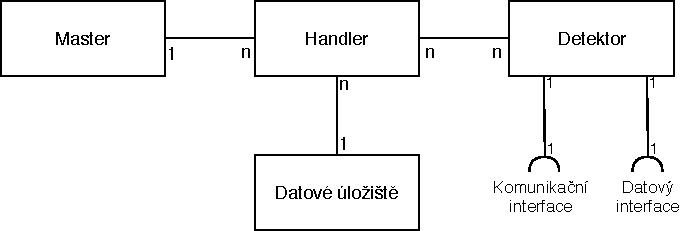
\includegraphics[width=14.5cm]{figures/arch_sw.pdf}
		\caption{Pixnet: softwarová architektura.}
		\label{fig:arch:sw_architecture}
	\end{center}
\end{figure}

V následujících podkapitolách budou detailněji popsány jednotlivé komponenty z obrázku~\ref{chap:arch:sw}.
\subsection{Detektor}\label{chap:arch:sw:detector}
Detektor je logická jednotka systému, která je reprezentována implementací komunikačního a datového interface, konfigurací a svým stavem. Fyzické propojení s detektorem je realizováno implementací komunikačního interface.

Komunikační interface obsahuje na příklad metody pro navazování spojení s detektorem, metody pro nahrávání konfigurace a metody pro získání podporovaných příkazů detektoru a jejich vykonání. Každý příkaz má svoje ID, název a model vstupních a výstupních hodnot. Modelem hodnot rozumíme množinu parametrů různých datových typů (\texttt{boolean}, \texttt{integer}, \texttt{float} apod.), které můžou nabývat hodnot omezených zadaným intervalem, nebo jedné z předdefinovaných diskrétních hodnot.

Datový interface obsahuje kromě inicializačních metod (předání konfigurace detektoru apod.) také metodu pro předání reference na asynchronní frontu naměřených dat, do které jsou data vkládána implementací komunikačního interface. Datový interface může mít několik implementací - na příklad data můžou být ukládána do datového úložiště handleru a následně asynchronně nahrána do centrálního datového úložiště, nebo můžou být rovnou synchronně nahrávána do datového úložiště.

\subsection{Datové úložiště}
Datové úložiště by mělo být škálovatelné, protože pro sítě o vetším počtu detektorů by ukládání dat do jednoho uzlu znamenalo omezení maximálního datového toku, dané kapacitou daného uzlu.

Jednou z možností implementace by mohlo být využití distribuovaného souborového systému, na příklad \textit{Hadoop Distributed File System} \cite{HDFS}, který se v praxi\footnote{Na příklad v roce 2010 internetová společnost \textit{Yahoo!} používala \texttt{HDFS} pro persistenci \unit{25}{PB} podnikových dat \cite{HDFS}.} používá pro distribuované ukládání dat s možností jejich redundance na více uzlech (pro potřeby zálohování). 

Další možností může být použití nějaké \texttt{NoSQL} distribuované databáze, na příklad \textit{MondoDB} \cite{mongodb-scale}. \textit{MondoDB} je dokumentová databáze, kde jednotlivé dokumenty jsou uloženy ve formátu \texttt{BSON}\footnote{Binární forma JSON (z ang. JavaScript Object Notation)}. Mezi hlavní výhody \textit{MondoDB} patří:
\begin{description}
    \item[Indexace:] Na každé pole objektů v dokumentu lze vytvořit index a tím zrychlit vyhledávání v datech.
    \item[Replikace:] \textit{MondoDB} ukládá data do tzv. \textit{replica set}, která obsahuje jednu, nebo více replik dat. Pro případ více replik, jedna vždy funguje jako primární a ostatní jako sekundární, do kterých jsou replikována data z primární repliky. Hlavní výhoda spočívá ve vyšší dostupnosti dat (data lze číst z více replik současně) a spolehlivosti (když jedna replika selže, je nahrazena replikou jinou).
    \item[Horizontální škálování:] \textit{MondoDB} má podporu pro horizontální škálování pomocí tzv. \textit{shardingu}. \textit{Sharded cluster} je pak množina uzlů s jednotlivými \textit{shardy}, kde každý obsahuje podmnožinu \textit{shardovaných} dat.
\end{description}

\subsection{Handler}
Handler je komponenta, kterou je řízena podmnožina detektorů detektorové sítě. K jednomu handleru je tedy možné připojit $n$ detektorů, kde $n$ je omezeno sumou datového toku přes všechny připojené detektory v závislosti na maximálním možném datovém toku handleru.

Handler komunikuje s detektorem pomocí dodané implementace jeho komunikačního interface a data detektorem vygenerovaná jsou pomocí implementace datového interface uloženy do datového úložiště, nebo zpracovány jiným způsobem.

Handler je zodpovědný za zavedení dodaných implementací komunikačního a datového interface do systému. Na příklad po přiřazení detektoru handleru, handler získá seznam podporovaných příkazů detektoru a poskytne je masteru. To systému umožňuje řízení heterogenní sítě detektorům homogenním způsobem, jak již bylo zmíněno v \ref{chap:arch:motivation}.

Aby mylo možné handlery, potažmo detektory, řídit centralizovaně, handler poskytuje \texttt{API}\footnote{Z angl. \textit{Application programming interface} (aplikační programové rozhraní).}. Pomocí \texttt{API} jsou jednotlivé handlery připojovány do systému, handlerům jsou přiřazovány a odebírány detektory, inicializuje se konfigurace detektorů a ji řízena akvizice dat.

\subsection{Master}
Master je centrální prvek systému, jehož prostřednictvím jsou řízeny handlery. Master poskytuje \texttt{API} pro své řízení pomocí pomocí frontendové aplikace. Tato aplikace je webový tenký klient, který uživateli poskytuje uživatelské rozhraní pro řízení systému.

Když na příklad uživatel přidává nový detektor do systému, tak nejprve skrze uživatelské rozhraní frontend aplikace zadá parametry detektoru, včetně implementace komunikačního a datového rozhraní, jak je znázorněno na obr. \ref{fig:arch:handler:new_detector}. Poté pomocí je detektor nahrán do mastera pomocí jeho \texttt{API}, kde je následně perzistentně uložen do jeho databáze. Při přiřazování detektoru handleru je konfigurace detektoru včetně implementace komunikačního a datového interface nahrána do zvoleného handleru, kde je dále zpracována. Zpracování konfigurace probíhá v následujících krocích:
\begin{enumerate}
    \item Vytvoření instance komunikačního interface a ověření jeho validity.
    \item Vytvoření instance datového interface a ověření jeho validity.
    \item Syntaktická analýza (tzv \textit{parsing}) konfigurace detektoru a její nahrání do instancích komunikačního a datového interface.
    \item Vytvoření asynchronní fronty měřených dat a její předání instancím komunikačního a datového interface.
\end{enumerate}
Po dokončení inicializační sekvence je uživatel notifikován a v případě úspěšného dokončení je detektor připraven vykonávat příchozí příkazy a měřit data.

\begin{figure}
	\begin{center}
		\begin{sequencediagram}
            \newthread[blue_ligh]{mf}{Master frontend}
            \newinst[0.5]{mb}{Master backend}
            \newinst[0.5]{h}{Handler}
            \newinst[0.5]{d}{Detektor}
            \newinst[0.19]{c}{\shortstack{Impl kom.\\interface}}
            \newinst[0.19]{p}{\shortstack{Impl dat.\\interface}}
            
            % nahrání konfigurace
            \postlevel
            \begin{call}{mf}{
                %pro úpravu thread color
                %\tikzset{threadstyle/.style={top color=white,bottom color=red}}
                    \shortstack{
                        Přidání nového\\
                        detektoru
                    }
                }{mb}{výsledek}
                
                \begin{callself}{mb}{\shortstack{Validace a uložení\\konfigurace detektoru}}{výsledek}
                \end{callself}	
                
            \end{call}

            % binding
            \postlevel
            \begin{call}{mf}{\shortstack{Přiřazení detektoru\\handleru}}{mb}{výsledek}
                
                \postlevel
                \begin{call}{mb}{\shortstack{Přiřazení\\detektoru}}{h}{výsledek}
                    
                    \begin{call}{h}{\shortstack{Inicializace}}{d}{výsledek}
                        
                        \begin{call}{d}{\shortstack{Zavedení\\modulu}}{c}{}
                        \end{call}
    
                        \begin{call}{d}{\shortstack{Zavedení modulu}}{p}{}
                        \end{call}

                        \postlevel
                        \begin{call}{d}{\shortstack{Nahrání\\konfigurace}}{c}{}
                        \end{call}

                        \begin{call}{d}{\shortstack{Nahrání konfigurace}}{p}{}
                        \end{call}
        
                        \begin{messcall}{d}{\shortstack{Fronta dat}}{c}
                        \end{messcall}

                        \begin{messcall}{d}{\shortstack{Fronta dat}}{p}
                        \end{messcall}
        
                    \end{call}
        
                \end{call}

            \end{call}
            
		\end{sequencediagram}
		\caption{Sekvenční diagram znázorňující příklad přidání detektoru do systému a jeho přiřazení handleru.}
		\label{fig:arch:handler:new_detector}
	\end{center}
\end{figure}

Jako datové úložiště pro konfigurace detektorů, informace o jejich stavu a o stavu jednotlivých handlerů bude navržena relační \texttt{SQL}\footnote{Z angl. \textit{Structured Query Language} (strukturovaný dotazovací jazyk).} databáze, ke které bude přistupovat pouze backend mastera.

\section{Hardwarová architektura}
V předchozí podkapitole byla popsána softwarová architektura. Fyzická instalace sítě přináší další omezení, především z pohledu síťové infrastruktury, které budou popsány v této podkapitole.

Na obrázku \ref{fig:arch:hw_architecture} je příklad sítě sestávající se ze dvou podsítí (tzv \textit{subnetwork}). Podsítí rozumíme takovou podmnožinu detektorů a handlerů, ve které libovolný detektor může být přiřazen libovolnému handleru. Pro úplnost je třeba doplnit, že nutnou podmínkou je, aby všechny handlery měly spojení s masterem a s distribuovaným úložištěm naměřených dat.

\begin{figure}[h]
	\begin{center}
		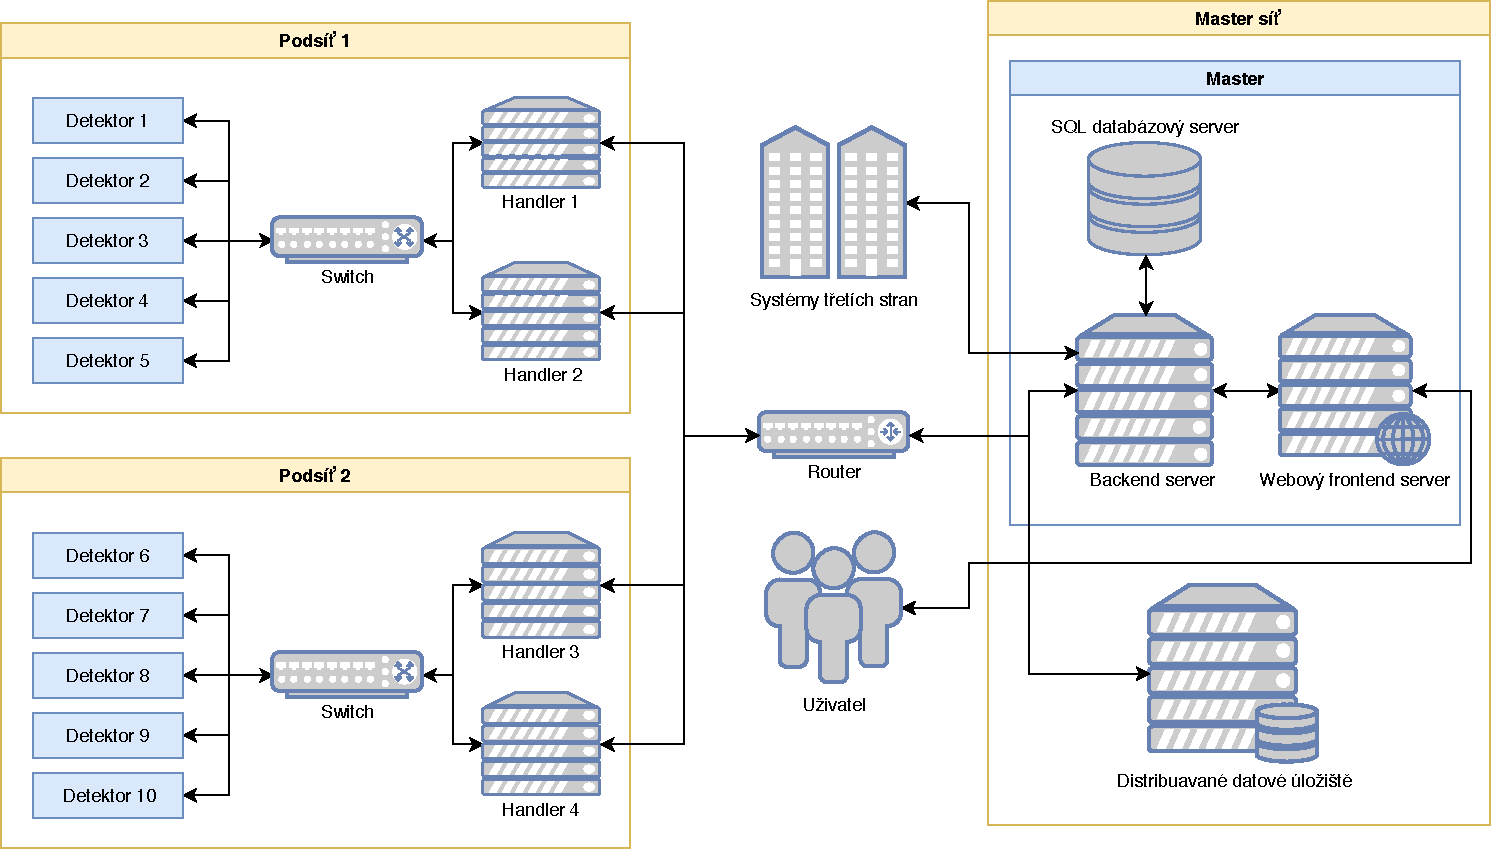
\includegraphics[width=15cm]{figures/arch_hw.pdf}
		\caption{Pixnet: hardwarová architektura s příkladem realizace sítě o dvou podsítích, kde v každé jsou dva handlery a pět detektorů, mastera (s \textit{SQL} databází pro persistenci konfigurace a frontend server poskytující webovou aplikaci) a centrálního datového úložiště naměřených dat.}
		\label{fig:arch:hw_architecture}
	\end{center}
\end{figure}

Master se skládá ze tří komponent:
\begin{description}
    \item[Backend serveru] implementujícího business logiku pro komunikaci s handlery (jako na příklad přiřazování detektorů, řízení akvizice dat apod.). Server zároveň poskytuje \textit{API} pro možnou integraci s webovým frontend serverem se systémy třetích stran\footnote{Na příklad pro experiment \textit{ATLAS TPX} v CERN je plánována integrace s \texttt{DAC} \cite{cern_dcs} (\textit{Detector control system}), který umožňuje centrální řízení detektorových systému, včetně integrace do bezpečnostního systému \texttt{DSS} (\textit{Detector safety system}), datového akvizičního systému \texttt{DAQ} (\textit{Data Acquisition System}) apod.}, kterými muže být plnohodnotně řízen.
    \item[Databázového serveru] poskytující relační \texttt{SQL} databázi pro persistenci konfigurace systému, včetně implementace potřebných rozhraní, stavových informací sítě apod.
    \item[Frontend serveru] poskytujícího webovou aplikaci s uživatelským rozhraním pro řízení mastera pomocí jeho \texttt{API}, resp. pro řízení celé sítě.
\end{description}

Na příkladu zmíněném výše je sít využívající jedno centrální datové úložiště. Realizace této komponenty je závislá na poskytnuté implementaci datových rozhraní jednotlivých detektorů. Může být implementovaná pomocí centralizovaného, nebo distribuovaného systému. Umístění úložiště také není omezeno - může být umístěno v sítě mastera, v jednotlivých podsítích, v síti mastera i v jednotlivých podsítích (buffer pro malou šířku pásma spojení podsíť - master síť), nebo třeba v internetu (cloudové úložiště, jako například \textit{Firebase Firestore}, \textit{Amazon 3S}, \textit{Microsoft Azure} apod.).

\section{Škálovatelnost}
\section{Použité technologie}


